\documentclass[a4paper, 12pt]{article}

% packages
\usepackage{amssymb}
\usepackage[fleqn]{mathtools}
\usepackage{tikz}
\usepackage{enumerate}
\usepackage{bussproofs}
\usepackage{xcolor}
\usepackage[margin=1.3cm]{geometry}
\usepackage{logicproof}
\usepackage{diagbox}
\usepackage{listings}
\usepackage{graphicx}
\usepackage{lstautogobble}
\usepackage{hyperref}
\usepackage{multirow}
\usepackage{tipa}
\usepackage{pgfplots}
\usepackage{adjustbox}

% tikz libraries
\usetikzlibrary{
    decorations.pathreplacing,
    arrows,
    shapes,
    shapes.gates.logic.US,
    circuits.logic.US,
    calc,
    automata,
    positioning,
    intersections
}

\pgfplotsset{compat=1.16}

\pgfmathdeclarefunction{gauss}{2}{%
  \pgfmathparse{1/(#2*sqrt(2*pi))*exp(-((x-#1)^2)/(2*#2^2))}%
}

\allowdisplaybreaks % allow environments to break
\setlength\parindent{0pt} % no indent

% shorthand for verbatim
% this clashes with logicproof, so maybe fix this at some point?
\catcode`~=\active
\def~#1~{\texttt{#1}}

% code listing
\lstdefinestyle{main}{
    numberstyle=\tiny,
    breaklines=true,
    showspaces=false,
    showstringspaces=false,
    tabsize=2,
    numbers=left,
    basicstyle=\ttfamily,
    columns=fixed,
    fontadjust=true,
    basewidth=0.5em,
    autogobble,
    xleftmargin=3.0ex,
    mathescape=true
}
\newcommand{\dollar}{\mbox{\textdollar}} %
\lstset{style=main}

% augmented matrix
\makeatletter
\renewcommand*\env@matrix[1][*\c@MaxMatrixCols c]{%
\hskip -\arraycolsep
\let\@ifnextchar\new@ifnextchar
\array{#1}}
\makeatother

% ceiling / floor
\DeclarePairedDelimiter{\ceil}{\lceil}{\rceil}
\DeclarePairedDelimiter{\floor}{\lfloor}{\rfloor}

% custom commands
\newcommand{\indefint}[2]{\int #1 \, \mathrm{d}#2}
\newcommand{\defint}[4]{\int_{#1}^{#2} #3 \, \mathrm{d}#4}
\newcommand{\pdif}[2]{\frac{\partial #1}{\partial #2}}
\newcommand{\dif}[2]{\frac{\mathrm{d}#1}{\mathrm{d}#2}}
\newcommand{\limit}[2]{\raisebox{0.5ex}{\scalebox{0.8}{$\displaystyle{\lim_{#1 \to #2}}$}}}
\newcommand{\limitsup}[2]{\raisebox{0.5ex}{\scalebox{0.8}{$\displaystyle{\limsup_{#1 \to #2}}$}}}
\newcommand{\summation}[2]{\sum\limits_{#1}^{#2}}
\newcommand{\product}[2]{\prod\limits_{#1}^{#2}}
\newcommand{\intbracket}[3]{\left[#3\right]_{#1}^{#2}}
\newcommand{\laplace}{\mathcal{L}}
\newcommand{\fourier}{\mathcal{F}}
\newcommand{\mat}[1]{\boldsymbol{#1}}
\renewcommand{\vec}[1]{\boldsymbol{#1}}
\newcommand{\rowt}[1]{\begin{bmatrix}
    #1
\end{bmatrix}^\top}
\DeclareMathOperator*{\argmax}{argmax}
\DeclareMathOperator*{\argmin}{argmin}

\newcommand{\lto}[0]{\leadsto\ }

\newcommand{\ulsmash}[1]{\underline{\smash{#1}}}

\newcommand{\powerset}[0]{\wp}
\renewcommand{\emptyset}[0]{\varnothing}

\makeatletter
\newsavebox{\@brx}
\newcommand{\llangle}[1][]{\savebox{\@brx}{\(\m@th{#1\langle}\)}%
  \mathopen{\copy\@brx\kern-0.5\wd\@brx\usebox{\@brx}}}
\newcommand{\rrangle}[1][]{\savebox{\@brx}{\(\m@th{#1\rangle}\)}%
  \mathclose{\copy\@brx\kern-0.5\wd\@brx\usebox{\@brx}}}
\makeatother
\newcommand{\lla}{\llangle}
\newcommand{\rra}{\rrangle}
\newcommand{\la}{\langle}
\newcommand{\ra}{\rangle}
\newcommand{\crnr}[1]{\text{\textopencorner} #1 \text{\textcorner}}
\newcommand{\bnfsep}[0]{\ |\ }
\newcommand{\concsep}[0]{\ ||\ }

\newcommand{\axiom}[1]{\AxiomC{#1}}
\newcommand{\unary}[1]{\UnaryInfC{#1}}
\newcommand{\binary}[1]{\BinaryInfC{#1}}
\newcommand{\trinary}[1]{\TrinaryInfC{#1}}
\newcommand{\quaternary}[1]{\QuaternaryInfC{#1}}
\newcommand{\quinary}[1]{\QuinaryInfC{#1}}
\newcommand{\dproof}[0]{\DisplayProof}
\newcommand{\llabel}[1]{\LeftLabel{\scriptsize #1}}
\newcommand{\rlabel}[1]{\RightLabel{\scriptsize #1}}

\newcommand{\ttbs}{\char`\\}
\newcommand{\lrbt}[0]{\ \bullet\ }

% colours
\newcommand{\violet}[1]{\textcolor{violet}{#1}}
\newcommand{\blue}[1]{\textcolor{blue}{#1}}
\newcommand{\red}[1]{\textcolor{red}{#1}}
\newcommand{\teal}[1]{\textcolor{teal}{#1}}

% reasoning proofs
\usepackage{ltablex}
\usepackage{environ}
\keepXColumns
\NewEnviron{reasoning}{
    \begin{tabularx}{\textwidth}{rlX}
        \BODY
    \end{tabularx}
}
\newcommand{\proofline}[3]{$(#1)$ & $#2$ & \hfill #3 \smallskip \\}
\newcommand{\proofarbitrary}[1]{& take arbitrary $#1$ \smallskip \\}
\newcommand{\prooftext}[1]{\multicolumn{3}{l}{#1} \smallskip \\}
\newcommand{\proofmath}[3]{$#1$ & = $#2$ & \hfill #3 \smallskip \\}
\newcommand{\prooftherefore}[1]{& $\therefore #1$ \smallskip \\}
\newcommand{\proofbc}[0]{\prooftext{\textbf{Base Case}}}
\newcommand{\proofis}[0]{\prooftext{\textbf{Inductive Step}}}

% ER diagrams
\newcommand{\nattribute}[4]{
    \node[draw, state, inner sep=0cm, minimum size=0.2cm, label=#3:{#4}] (#1) at (#2) {};
}
\newcommand{\mattribute}[4]{
    \node[draw, state, accepting, inner sep=0cm, minimum size=0.2cm, label=#3:{#4}] (#1) at (#2) {};
}
\newcommand{\dattribute}[4]{
    \node[draw, state, dashed, inner sep=0cm, minimum size=0.2cm, label=#3:{#4}] (#1) at (#2) {};
}
\newcommand{\entity}[3]{
    \node[] (#1-c) at (#2) {#3};
    \node[inner sep=0cm] (#1-l) at ($(#1-c) + (-1, 0)$) {};
    \node[inner sep=0cm] (#1-r) at ($(#1-c) + (1, 0)$) {};
    \node[inner sep=0cm] (#1-u) at ($(#1-c) + (0, 0.5)$) {};
    \node[inner sep=0cm] (#1-d) at ($(#1-c) + (0, -0.5)$) {};
    \draw
    ($(#1-c) + (-1, 0.5)$) -- ($(#1-c) + (1, 0.5)$) -- ($(#1-c) + (1, -0.5)$) -- ($(#1-c) + (-1, -0.5)$) -- cycle;
}
\newcommand{\relationship}[3]{
    \node[] (#1-c) at (#2) {#3};
    \node[inner sep=0cm] (#1-l) at ($(#1-c) + (-1, 0)$) {};
    \node[inner sep=0cm] (#1-r) at ($(#1-c) + (1, 0)$) {};
    \node[inner sep=0cm] (#1-u) at ($(#1-c) + (0, 1)$) {};
    \node[inner sep=0cm] (#1-d) at ($(#1-c) + (0, -1)$) {};
    \draw
    ($(#1-c) + (-1, 0)$) -- ($(#1-c) + (0, 1)$) -- ($(#1-c) + (1, 0)$) -- ($(#1-c) + (0, -1)$) -- cycle;
}

% AVL Trees
\newcommand{\avltri}[4]{
    \draw ($(#1)$) -- ($(#1) + #4*(0.5, -1)$) -- ($(#1) + #4*(-0.5, -1)$) -- cycle;
    \node at ($(#1) + #4*(0, -1) + (0, 0.5)$) {#3};
    \node at ($(#1) + #4*(0, -1) + (0, -0.5)$) {#2};
}

% RB Trees
\tikzset{rbtr/.style={inner sep=2pt, circle, draw=black, fill=red}}
\tikzset{rbtb/.style={inner sep=2pt, circle, draw=black, fill=black}}

% Samples
\tikzset{spos/.style={inner sep=2pt, circle, draw=black, fill=blue!20}}
\tikzset{sneg/.style={inner sep=2pt, circle, draw=black, fill=red!20}}

% Joins
\newcommand\ljoin{\stackrel{\mathclap{\normalfont\mbox{\tiny L}}}{\bowtie}}
\newcommand\rjoin{\stackrel{\mathclap{\normalfont\mbox{\tiny R}}}{\bowtie}}
\newcommand\ojoin{\stackrel{\mathclap{\normalfont\mbox{\tiny O}}}{\bowtie}}

\setcounter{MaxMatrixCols}{100}

% actual document
\begin{document}
    {\sc Computing $3^\text{rd}$ Year Notes} \hfill ~https://github.com/lin-e/imperial-revision~
    \rule{\textwidth}{0.1pt}
    \section*{CO395 - Introduction to Machine Learning \hfill (70050)}
        \subsection*{Week 2 (Introduction to ML)}
        \subsection*{Week 3 (Instance-based Learning + Decision Trees)}
            The \textbf{k Nearest Neighbours (k-NN)} classifier is classified as a \textbf{lazy learner}.
            A lazy learner stores all the training examples in the data set, and postpone any processing until a request is made (such as a prediction).
            On the other hand, \textbf{decision trees} are classified as a \textbf{eager learner}.
            An eager learner will attempt to construct a general target decision function, which is prepared prior to a query being made.
            \subsubsection*{Classification with Instance-based Learning}
                The concept behind instance-based learning is that we will use samples in a training data set in order to make inference on a query.
                \medskip

                The \textbf{Nearest Neighbour} classifier is a specific example, where it classifies a test instance to the label of the nearest training instance, where nearest is subject to some distance metric.
                This is a \textbf{non-parametric model}, which means it naturally emerges from the training set.
                Note in the example below, an issue with this is that it can be sensitive to noise, as it would classify the \blue{blue} point to be \red{red}, as it is the closest instance in the training set, even though it's more likely to be black - it is very sensitive to noise, and can \textbf{overfit} to the training data.
                \medskip

                On the other hand, if we consider the \textbf{k Nearest Neighbours}, highlighted by the lines in \violet{violet}, we get the class to be black, as we have 4 against 1.
                Usually, we need $k$ to be odd, to ensure a winner for the decision task.
                \begin{center}
                    \begin{tikzpicture}[x=1.5cm]
                        % using CO202's RBT nodes because I'm lazy
                        \node[rbtr] at (0, 0) {};
                        \node[rbtr] at (-3, -1) {};
                        \node[rbtr] at (-1, -1) {};
                        \node[rbtr] at (-2, -2) {};
                        \node[rbtr] at (-3, -3) {};
                        \node[rbtr] at (-1, -3) {};
                        \node[rbtb] at (-2, -4) {};
                        \node[rbtb] at (0, -4) {};
                        \node[rbtb] at (1, -4) {};
                        \node[rbtb] (nn4) at (2, -3) {};
                        \node[rbtr] (nn0) at (2, -2) {};
                        \node[inner sep=2pt, circle, draw=black, fill=blue] (test) at (1, -2) {};
                        \node[rbtb] (nn1) at (1, -0.5) {};
                        \node[rbtb] (nn2) at (1, -3.5) {};
                        \node[rbtb] (nn3) at (2, -1) {};
                        \node[rbtb] at (3, -1) {};
                        \node[rbtb] at (3, -2) {};
                        \node[rbtb] at (4, -2) {};
                        \node[rbtb] at (5, 0) {};

                        \draw
                        (test) edge[dashed] (nn0)
                        (test) edge[dashed, violet] (nn1)
                        (test) edge[dashed, violet] (nn2)
                        (test) edge[dashed, violet] (nn3)
                        (test) edge[dashed, violet] (nn4);
                    \end{tikzpicture}
                \end{center}
                Increasing $k$ will give the classifier have a smoother decision boundary (higher bias), and less sensitive to training data (lower variance).
                Choosing $k$ is dependant on the dataset, normally with a validation dataset.
                \medskip

                The distance metric can be defined in many different ways, including the $\ell_1$, $\ell_2$ and $\ell_\infty$-norms as seen in \textbf{CO233}.
                Other metrics exist such as the \textbf{Mahalanobis distance} for non-isotropic spaces, typically used for Gaussian distributions, or the \textbf{Hamming distance} for binary strings.
                \medskip

                Another variation is the \textbf{Distance Weighted k-NN}.
                For example, we may not want to trust neighbours which are further away, such as in the example below.
                \begin{center}
                    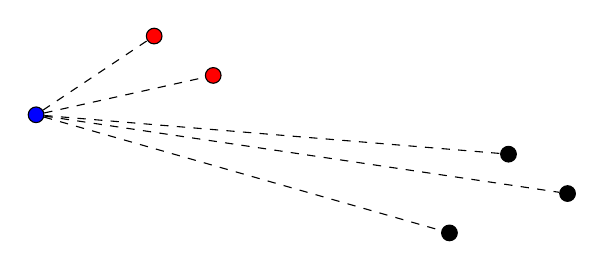
\begin{tikzpicture}[x=1.5cm]
                        \node[inner sep=2pt, circle, draw=black, fill=blue] (test) at (0, 0) {};
                        \node[rbtr] (nn0) at (1, 1) {};
                        \node[rbtr] (nn1) at (1.5, 0.5) {};
                        \node[rbtb] (nn2) at (4, -0.5) {};
                        \node[rbtb] (nn3) at (3.5, -1.5) {};
                        \node[rbtb] (nn4) at (4.5, -1) {};

                        \draw
                        (test) edge[dashed] (nn0)
                        (test) edge[dashed] (nn1)
                        (test) edge[dashed] (nn2)
                        (test) edge[dashed] (nn3)
                        (test) edge[dashed] (nn4);
                    \end{tikzpicture}
                    \hfill
                    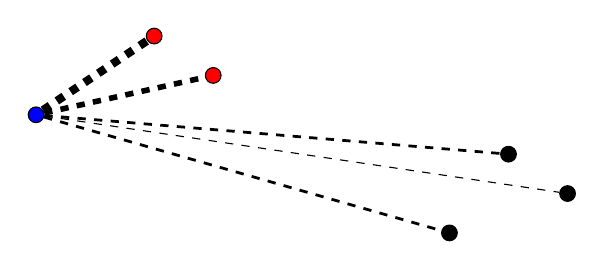
\begin{tikzpicture}[x=1.5cm]
                        \node[inner sep=2pt, circle, draw=black, fill=blue] (test) at (0, 0) {};
                        \node[rbtr] (nn0) at (1, 1) {};
                        \node[rbtr] (nn1) at (1.5, 0.5) {};
                        \node[rbtb] (nn2) at (4, -0.5) {};
                        \node[rbtb] (nn3) at (3.5, -1.5) {};
                        \node[rbtb] (nn4) at (4.5, -1) {};

                        \draw
                        (test) edge[dashed, line width=3pt] (nn0)
                        (test) edge[dashed, line width=2pt] (nn1)
                        (test) edge[dashed, line width=1pt] (nn2)
                        (test) edge[dashed, line width=1pt] (nn3)
                        (test) edge[dashed] (nn4);
                    \end{tikzpicture}
                \end{center}
                The idea is that we add weights to each neighbour (depending on distance), typically a higher weight for closer neighbours.
                We then assign the class based on which class has the largest sum.
                This metric, $w^{(i)}$, is any measure favouring the votes of nearby neighbours, such as;
                \begin{itemize}
                    \itemsep0em
                    \item inverse of distance
                        \[w^{(i)} = \frac{1}{d(x^{(i)}, x^{(q)})}\]
                    \item Gaussian distribution
                        \[w^{(i)} = \frac{1}{\sqrt{2 \pi}}e^{-\frac{d\left(x^{(i)}, x^{(q)}\right)^2}{2}}\]
                \end{itemize}
                The value of $k$ is less important in the weighted case, as distant examples won't greatly affect classification.
                If $k = N$, where $N$ is the size of the training set, it is a global method, otherwise it is a local method (only considering the samples close by).
                This method is also more robust to noisy training data, however it can be slow for large datasets.
                \medskip

                As this method relies on distance metrics, it may not work well if using all features in high dimensional spaces.
                If these features are irrelevant, instances in the same class may be far from each other.
                One solution to this is to weight features differently.
                \medskip

                k-NN can also be used for regression, either by computing the mean value across $k$ nearest neighbours (which leads to a very rough curve), or by using locally weighted regression, which computes the weighted mean value across $k$ nearest neighbours, leading to a smoother curve.
            \subsubsection*{Classification with Decision Trees}
                Decisions trees are the principal of focusing on a subset or single feature of each sample and then make a decision whether it's true or false (for each feature), and repeat this process to finer decisions until we manage to classify the sample that we want to check.
                \medskip

                In decision trees, we learn a succession of linear decision boundaries that we can use to eventually correctly classify samples.
                \begin{center}
                    \hfill
                    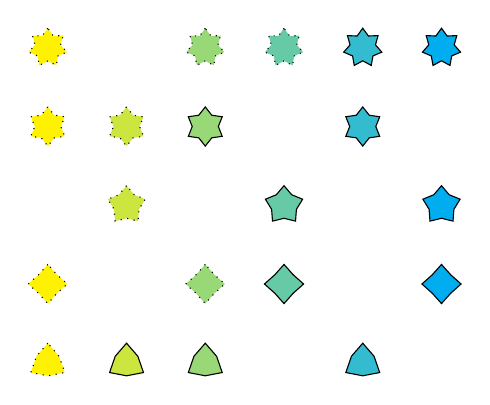
\begin{tikzpicture}
                        \node[dotted, draw, star, star points=3, fill=yellow!100!cyan] at (0, 0) {};
                        \node[dotted, draw, star, star points=4, fill=yellow!100!cyan] at (0, 1) {};
                        \node[dotted, draw, star, star points=6, fill=yellow!100!cyan] at (0, 3) {};
                        \node[dotted, draw, star, star points=7, fill=yellow!100!cyan] at (0, 4) {};

                        \node[draw, star, star points=3, fill=yellow!80!cyan] at (1, 0) {};
                        \node[dotted, draw, star, star points=5, fill=yellow!80!cyan] at (1, 2) {};
                        \node[dotted, draw, star, star points=6, fill=yellow!80!cyan] at (1, 3) {};

                        \node[draw, star, star points=3, fill=yellow!60!cyan] at (2, 0) {};
                        \node[dotted, draw, star, star points=4, fill=yellow!60!cyan] at (2, 1) {};
                        \node[draw, star, star points=6, fill=yellow!60!cyan] at (2, 3) {};
                        \node[dotted, draw, star, star points=7, fill=yellow!60!cyan] at (2, 4) {};

                        \node[draw, star, star points=4, fill=yellow!40!cyan] at (3, 1) {};
                        \node[draw, star, star points=5, fill=yellow!40!cyan] at (3, 2) {};
                        \node[dotted, draw, star, star points=7, fill=yellow!40!cyan] at (3, 4) {};

                        \node[draw, star, star points=3, fill=yellow!20!cyan] at (4, 0) {};
                        \node[draw, star, star points=6, fill=yellow!20!cyan] at (4, 3) {};
                        \node[draw, star, star points=7, fill=yellow!20!cyan] at (4, 4) {};

                        \node[draw, star, star points=4, fill=yellow!0!cyan] at (5, 1) {};
                        \node[draw, star, star points=5, fill=yellow!0!cyan] at (5, 2) {};
                        \node[draw, star, star points=7, fill=yellow!0!cyan] at (5, 4) {};
                    \end{tikzpicture}
                    \hfill
                    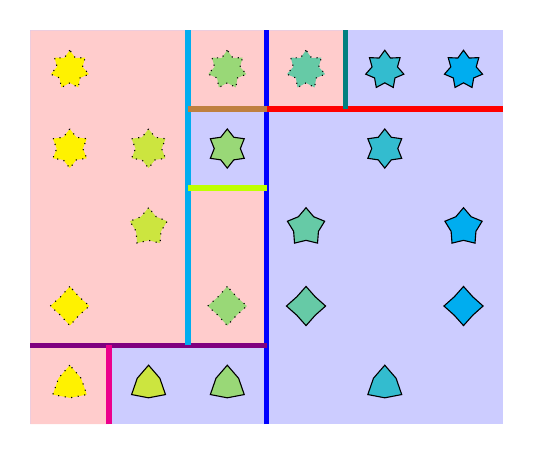
\begin{tikzpicture}
                        \fill[blue!20]
                        (-0.5, -0.5) -- (-0.5, 4.5) -- (5.5, 4.5) -- (5.5, -0.5) -- cycle;
                        \fill[red!20]
                        (-0.5, -0.5) -- (-0.5, 4.5) -- (3.5, 4.5) -- (3.5, 3.5) -- (1.5, 3.5) -- (1.5, 2.5) --(2.5, 2.5) -- (2.5, 0.5) -- (0.5, 0.5) -- (0.5, -0.5) -- cycle;
                        \node[dotted, draw, star, star points=3, fill=yellow!100!cyan] at (0, 0) {};
                        \node[dotted, draw, star, star points=4, fill=yellow!100!cyan] at (0, 1) {};
                        \node[dotted, draw, star, star points=6, fill=yellow!100!cyan] at (0, 3) {};
                        \node[dotted, draw, star, star points=7, fill=yellow!100!cyan] at (0, 4) {};

                        \node[draw, star, star points=3, fill=yellow!80!cyan] at (1, 0) {};
                        \node[dotted, draw, star, star points=5, fill=yellow!80!cyan] at (1, 2) {};
                        \node[dotted, draw, star, star points=6, fill=yellow!80!cyan] at (1, 3) {};

                        \node[draw, star, star points=3, fill=yellow!60!cyan] at (2, 0) {};
                        \node[dotted, draw, star, star points=4, fill=yellow!60!cyan] at (2, 1) {};
                        \node[draw, star, star points=6, fill=yellow!60!cyan] at (2, 3) {};
                        \node[dotted, draw, star, star points=7, fill=yellow!60!cyan] at (2, 4) {};

                        \node[draw, star, star points=4, fill=yellow!40!cyan] at (3, 1) {};
                        \node[draw, star, star points=5, fill=yellow!40!cyan] at (3, 2) {};
                        \node[dotted, draw, star, star points=7, fill=yellow!40!cyan] at (3, 4) {};

                        \node[draw, star, star points=3, fill=yellow!20!cyan] at (4, 0) {};
                        \node[draw, star, star points=6, fill=yellow!20!cyan] at (4, 3) {};
                        \node[draw, star, star points=7, fill=yellow!20!cyan] at (4, 4) {};

                        \node[draw, star, star points=4, fill=yellow!0!cyan] at (5, 1) {};
                        \node[draw, star, star points=5, fill=yellow!0!cyan] at (5, 2) {};
                        \node[draw, star, star points=7, fill=yellow!0!cyan] at (5, 4) {};

                        \draw[blue, line width=2pt] (2.5, -0.5) -- (2.5, 4.5);
                        \draw[red, line width=2pt] (2.5, 3.5) -- (5.5, 3.5);
                        \draw[violet, line width=2pt] (-0.5, 0.5) -- (2.5, 0.5);
                        \draw[teal, line width=2pt] (3.5, 3.5) -- (3.5, 4.5);
                        \draw[magenta, line width=2pt] (0.5, -0.5) -- (0.5, 0.5);
                        \draw[cyan, line width=2pt] (1.5, 0.5) -- (1.5, 4.5);
                        \draw[lime, line width=2pt] (1.5, 2.5) -- (2.5, 2.5);
                        \draw[brown, line width=2pt] (1.5, 3.5) -- (2.5, 3.5);
                    \end{tikzpicture}
                    \hfill
                    \phantom{}
                \end{center}
                In the example above, we repeatedly choose divisions that result in the fewest number of errors, until we are able to classify everything.
                This results in the following decision tree, when we are using the attributes of colour and number of points.
                For brevity, the left branch is the ~false~ branch, ~p~ means points, and ~c~ means colour.
                \begin{center}
                    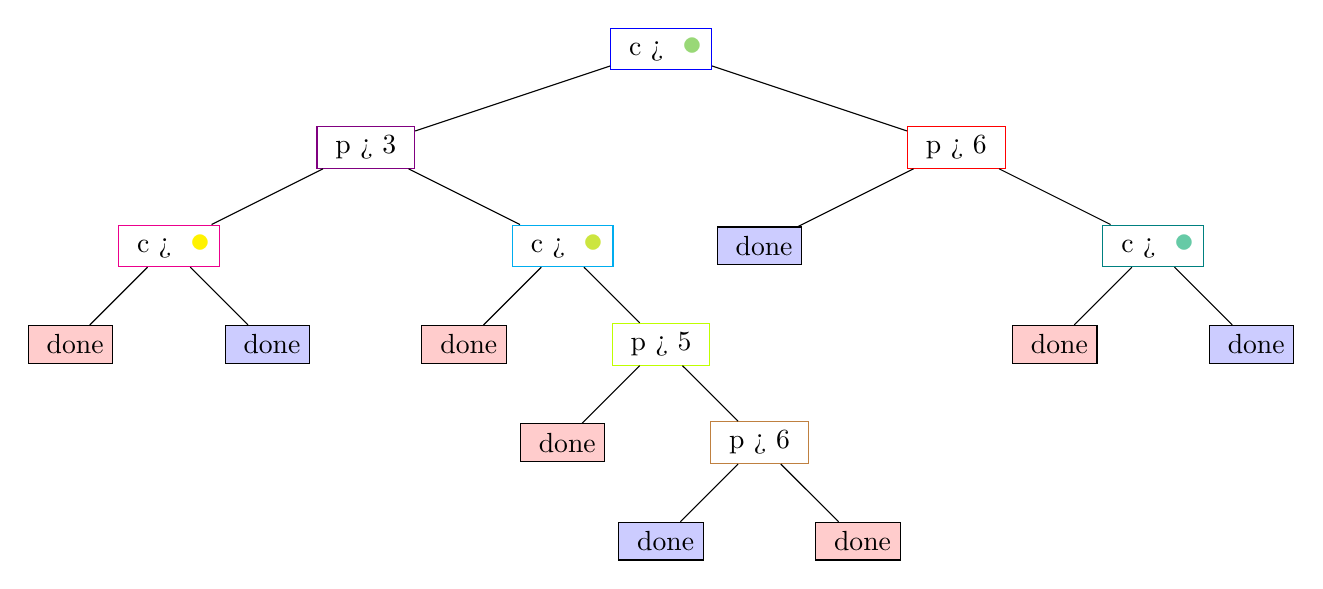
\begin{tikzpicture}[x=1.25cm, y=1.25cm]
                        \node[draw, blue] (o) at (0, 0) {\textcolor{black}{~c > ~}\textcolor{yellow!60!cyan}{\Large$\bullet$}};
                        \node[draw, violet] (ol) at (-3, -1) {\textcolor{black}{~p > 3~}};
                        \node[draw, magenta] (oll) at (-5, -2) {\textcolor{black}{~c > ~}\textcolor{yellow!100!cyan}{\Large$\bullet$}};
                        \node[draw, fill=red!20] (olll) at (-6, -3) {~done~};
                        \node[draw, fill=blue!20] (ollr) at (-4, -3) {~done~};
                        \node[draw, cyan] (olr) at (-1, -2) {\textcolor{black}{~c > ~}\textcolor{yellow!80!cyan}{\Large$\bullet$}};
                        \node[draw, fill=red!20] (olrl) at (-2, -3) {~done~};
                        \node[draw, lime] (olrr) at (0, -3) {\textcolor{black}{~p > 5~}};
                        \node[draw, fill=red!20] (olrrl) at (-1, -4) {~done~};
                        \node[draw, brown] (olrrr) at (1, -4) {\textcolor{black}{~p > 6~}};
                        \node[draw, fill=blue!20] (olrrrl) at (0, -5) {~done~};
                        \node[draw, fill=red!20] (olrrrr) at (2, -5) {~done~};
                        \node[draw, red] (or) at (3, -1) {\textcolor{black}{~p > 6~}};
                        \node[draw, fill=blue!20] (orl) at (1, -2) {~done~};
                        \node[draw, teal] (orr) at (5, -2) {\textcolor{black}{~c > ~}\textcolor{yellow!40!cyan}{\Large$\bullet$}};
                        \node[draw, fill=red!20] (orrl) at (4, -3) {~done~};
                        \node[draw, fill=blue!20] (orrr) at (6, -3) {~done~};

                        \draw
                        (o) -- (ol)
                        (o) -- (or)
                        (ol) -- (oll)
                        (ol) -- (olr)
                        (or) -- (orl)
                        (or) -- (orr)
                        (oll) -- (olll)
                        (oll) -- (ollr)
                        (olr) -- (olrl)
                        (olr) -- (olrr)
                        (orr) -- (orrl)
                        (orr) -- (orrr)
                        (olrr) -- (olrrl)
                        (olrr) -- (olrrr)
                        (olrrr) -- (olrrrl)
                        (olrrr) -- (olrrrr);
                    \end{tikzpicture}
                \end{center}
                Decision trees are a method of approximating discrete classification functions, by representing them as a tree (a set of if-then rules).
                The general algorithm (ID3) for constructing a decision tree is as follows;
                \begin{enumerate}[1.]
                    \itemsep0em
                    \item search for the optimal splitting rule on training data
                    \item split data according to rule
                    \item repeat 1 and 2 on each subset until each subset is pure (only containing a single class)
                \end{enumerate}
            \subsubsection*{How to select the `optimal' split rule}
                Intuitively, we want to partition the datasets such that they are more pure than the original set.
                To do this, we have several metrics;
                \begin{itemize}
                    \itemsep0em
                    \item \textbf{Information gain} \hfill ID3, C4.5
                        \subitem quantifies the reduction of \textbf{entropy}
                    \item \textbf{Gini impurity} \hfill CART
                        \subitem if we randomly select a point in the feature space and randomly classify it according to the class label distribution, what is our probability of getting it incorrect?
                    \item \textbf{Variance reduction} \hfill CART
                        \subitem mostly used for regression trees, with a continuous target variable
                \end{itemize}
                To do this, we need to understand information entropy.
                Entropy is a measure of uncertainty of a random variable.
                It can also be seen as the average amount of information needed to define a random state / variable.
                If something has low entropy, it's predictable, and vice versa for high entropy.
                \medskip

                Imagine we have two boxes, with something stored in one of the two, with an equal probability in each.
                To be fully certain, we need a single bit of information, if it's in the left box, the bit is ~0~, otherwise (if it's in the right box), it's ~1~.
                Similarly, if we have four boxes, with a uniform distribution, we would need 4 bits to encode the 4 states.
                In general;
                \begin{align*}
                    2^B & = K \text{ states} \\
                    B & = \log_2(K) \\
                    I(x) & = \log_2(K) & \text{amount of information to determine the state of a random variable} \\
                    P(x) & = \frac{1}{K} & \Rightarrow \\
                    K & = \frac{1}{K} & \Rightarrow \\
                    I(x) & = -\log_2(P(x))
                \end{align*}
                As such, we can say;
                $$I(x = \text{box}_1) = I(x = \text{box}_2) = I(x = \text{box}_3) = I(x = \text{box}_4) = -\log_2(P(x)) = 2 \text{ bits}$$
                However, assume a non-uniform distribution, with the probabilities being 97\%, 1\%, 1\%, and 1\% respectively.
                If we were told it was in box 1, we do not get a lot of new information (low entropy); however if we were told it was in one of the other three, we high entropy (represents very important information).
                \begin{align*}
                    I(x = \text{box}_1) & = -\log_2(0.97) \\
                    & \approx 0.0439 \text{ bits} \\
                    I(x = \text{box}_2) & = -\log_2(0.1) \\
                    & \approx 6.6439 \text{ bits}
                \end{align*}
                Entropy is defined as the average amount of information;
                $$H(X) = -\summation{k}{K}P(x_k)\log_2(P(x_k))$$
                In our example, we therefore have;
                $$H(X) = -(0.97 \cdot \log_2(0.97) + 0.01 \cdot \log_2(0.01) + 0.01 \cdot \log_2(0.01) + 0.01 \cdot \log_2(0.01)) \approx 0.2419 \text{ bits}$$
                We therefore need, on average, less information to know where the key is (compared to the uniform distribution).
                \medskip

                For continuous entropy, we can use the probability density function $f(x)$ - this is imperfect (it can have negative values), but is still often used in Deep Learning.;
                $$H(X) = - \defint{x}{}{f(x)\log_2(f(x))}{x}$$
                Consider the following example;
                \begin{center}
                    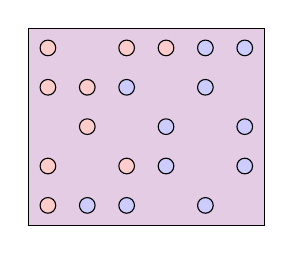
\begin{tikzpicture}[x=0.5cm, y=0.5cm]
                        \draw[fill=violet!20] (-0.5, -0.5) -- (-0.5, 4.5) -- (5.5, 4.5) -- (5.5, -0.5) -- cycle;

                        \node[sneg] at (0, 0) {};
                        \node[sneg] at (0, 1) {};
                        \node[sneg] at (0, 3) {};
                        \node[sneg] at (0, 4) {};

                        \node[spos] at (1, 0) {};
                        \node[sneg] at (1, 2) {};
                        \node[sneg] at (1, 3) {};

                        \node[spos] at (2, 0) {};
                        \node[sneg] at (2, 1) {};
                        \node[spos] at (2, 3) {};
                        \node[sneg] at (2, 4) {};

                        \node[spos] at (3, 1) {};
                        \node[spos] at (3, 2) {};
                        \node[sneg] at (3, 4) {};

                        \node[spos] at (4, 0) {};
                        \node[spos] at (4, 3) {};
                        \node[spos] at (4, 4) {};

                        \node[spos] at (5, 1) {};
                        \node[spos] at (5, 2) {};
                        \node[spos] at (5, 4) {};
                    \end{tikzpicture}
                    \begin{align*}
                        P(\textcolor{blue!20}{\bullet}) & = \frac{11}{20} \\
                        P(\textcolor{red!20}{\bullet}) & = \frac{9}{20} \\
                        H(\textcolor{violet!20}{\blacksquare}) & = -\left(\frac{11}{20} \cdot \log_2\left(\frac{11}{20}\right) + \frac{9}{20} \cdot \log_2\left(\frac{9}{20}\right)\right) \\
                        & \approx 0.9928
                    \end{align*}
                \end{center}
                An entropy value close to 1 would indicate a maximum amount of information needed.
                \begin{center}
                    \hfill
                    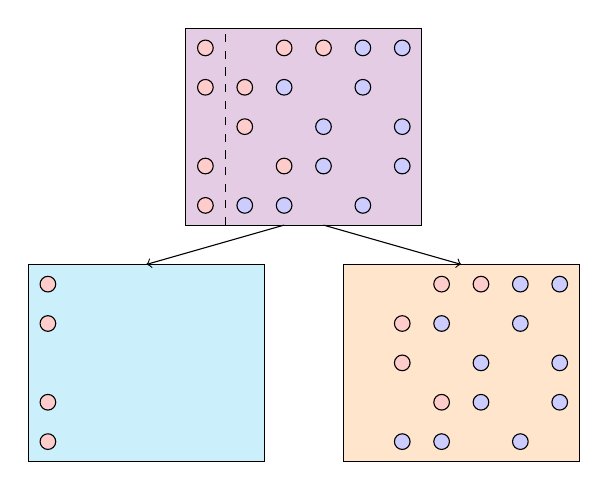
\begin{tikzpicture}[x=0.5cm, y=0.5cm]
                        \begin{scope}[shift={(0, 0)}]
                            \draw[fill=violet!20] (-0.5, -0.5) -- (-0.5, 4.5) -- (5.5, 4.5) -- (5.5, -0.5) -- cycle;

                            \node[sneg] at (0, 0) {};
                            \node[sneg] at (0, 1) {};
                            \node[sneg] at (0, 3) {};
                            \node[sneg] at (0, 4) {};

                            \node[spos] at (1, 0) {};
                            \node[sneg] at (1, 2) {};
                            \node[sneg] at (1, 3) {};

                            \node[spos] at (2, 0) {};
                            \node[sneg] at (2, 1) {};
                            \node[spos] at (2, 3) {};
                            \node[sneg] at (2, 4) {};

                            \node[spos] at (3, 1) {};
                            \node[spos] at (3, 2) {};
                            \node[sneg] at (3, 4) {};

                            \node[spos] at (4, 0) {};
                            \node[spos] at (4, 3) {};
                            \node[spos] at (4, 4) {};

                            \node[spos] at (5, 1) {};
                            \node[spos] at (5, 2) {};
                            \node[spos] at (5, 4) {};

                            \draw (0.5, -0.5) edge[dashed] (0.5, 4.5);
                        \end{scope}
                        \begin{scope}[shift={(-4, -6)}]
                            \draw (-0.5, -0.5)[fill=cyan!20] -- (-0.5, 4.5) -- (5.5, 4.5) -- (5.5, -0.5) -- cycle;

                            \node[sneg] at (0, 0) {};
                            \node[sneg] at (0, 1) {};
                            \node[sneg] at (0, 3) {};
                            \node[sneg] at (0, 4) {};
                        \end{scope}
                        \begin{scope}[shift={(4, -6)}]
                            \draw (-0.5, -0.5)[fill=orange!20] -- (-0.5, 4.5) -- (5.5, 4.5) -- (5.5, -0.5) -- cycle;
                            \node[spos] at (1, 0) {};
                            \node[sneg] at (1, 2) {};
                            \node[sneg] at (1, 3) {};

                            \node[spos] at (2, 0) {};
                            \node[sneg] at (2, 1) {};
                            \node[spos] at (2, 3) {};
                            \node[sneg] at (2, 4) {};

                            \node[spos] at (3, 1) {};
                            \node[spos] at (3, 2) {};
                            \node[sneg] at (3, 4) {};

                            \node[spos] at (4, 0) {};
                            \node[spos] at (4, 3) {};
                            \node[spos] at (4, 4) {};

                            \node[spos] at (5, 1) {};
                            \node[spos] at (5, 2) {};
                            \node[spos] at (5, 4) {};
                        \end{scope}

                        \draw
                        (2, -0.5) edge[->] (-1.5, -1.5)
                        (3, -0.5) edge[->] (6.5, -1.5);
                    \end{tikzpicture}
                    \hfill
                    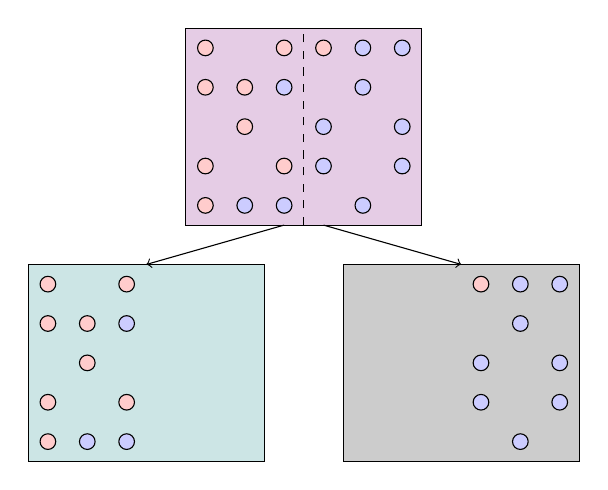
\begin{tikzpicture}[x=0.5cm, y=0.5cm]
                        \begin{scope}[shift={(0, 0)}]
                            \draw[fill=violet!20] (-0.5, -0.5) -- (-0.5, 4.5) -- (5.5, 4.5) -- (5.5, -0.5) -- cycle;

                            \node[sneg] at (0, 0) {};
                            \node[sneg] at (0, 1) {};
                            \node[sneg] at (0, 3) {};
                            \node[sneg] at (0, 4) {};

                            \node[spos] at (1, 0) {};
                            \node[sneg] at (1, 2) {};
                            \node[sneg] at (1, 3) {};

                            \node[spos] at (2, 0) {};
                            \node[sneg] at (2, 1) {};
                            \node[spos] at (2, 3) {};
                            \node[sneg] at (2, 4) {};

                            \node[spos] at (3, 1) {};
                            \node[spos] at (3, 2) {};
                            \node[sneg] at (3, 4) {};

                            \node[spos] at (4, 0) {};
                            \node[spos] at (4, 3) {};
                            \node[spos] at (4, 4) {};

                            \node[spos] at (5, 1) {};
                            \node[spos] at (5, 2) {};
                            \node[spos] at (5, 4) {};

                            \draw (2.5, -0.5) edge[dashed] (2.5, 4.5);
                        \end{scope}
                        \begin{scope}[shift={(-4, -6)}]
                            \draw[fill=teal!20] (-0.5, -0.5) -- (-0.5, 4.5) -- (5.5, 4.5) -- (5.5, -0.5) -- cycle;

                            \node[sneg] at (0, 0) {};
                            \node[sneg] at (0, 1) {};
                            \node[sneg] at (0, 3) {};
                            \node[sneg] at (0, 4) {};

                            \node[spos] at (1, 0) {};
                            \node[sneg] at (1, 2) {};
                            \node[sneg] at (1, 3) {};

                            \node[spos] at (2, 0) {};
                            \node[sneg] at (2, 1) {};
                            \node[spos] at (2, 3) {};
                            \node[sneg] at (2, 4) {};
                        \end{scope}
                        \begin{scope}[shift={(4, -6)}]
                            \draw[fill=black!20] (-0.5, -0.5) -- (-0.5, 4.5) -- (5.5, 4.5) -- (5.5, -0.5) -- cycle;

                            \node[spos] at (3, 1) {};
                            \node[spos] at (3, 2) {};
                            \node[sneg] at (3, 4) {};

                            \node[spos] at (4, 0) {};
                            \node[spos] at (4, 3) {};
                            \node[spos] at (4, 4) {};

                            \node[spos] at (5, 1) {};
                            \node[spos] at (5, 2) {};
                            \node[spos] at (5, 4) {};
                        \end{scope}

                        \draw
                        (2, -0.5) edge[->] (-1.5, -1.5)
                        (3, -0.5) edge[->] (6.5, -1.5);
                    \end{tikzpicture}
                    \hfill
                    \phantom{}
                \end{center}
                \begin{align*}
                    H(\textcolor{cyan!20}{\blacksquare}) & = 0 \\
                    H(\textcolor{orange!20}{\blacksquare}) & \approx 0.896 \\
                    H(\{\textcolor{cyan!20}{\blacksquare}, \textcolor{orange!20}{\blacksquare}\}) & \approx \frac{4}{20} \cdot 0 + \frac{16}{20} \cdot 0.896 \\
                    & \approx 0.7168 \\
                    H(\textcolor{violet!20}{\blacksquare}) - H(\{\textcolor{cyan!20}{\blacksquare}, \textcolor{orange!20}{\blacksquare}\}) & \approx 0.276 & \text{information gain} \\ \\
                    H(\textcolor{teal!20}{\blacksquare}) & \approx 0.8454 \\
                    H(\textcolor{black!20}{\blacksquare}) & \approx 0.5033 \\
                    H(\{\textcolor{teal!20}{\blacksquare}, \textcolor{black!20}{\blacksquare}\}) & \approx \frac{11}{20} \cdot 0.8454 + \frac{9}{20} \cdot 0.5033 \\
                    & \approx 0.6915 \\
                    H(\textcolor{violet!20}{\blacksquare}) - H(\{\textcolor{teal!20}{\blacksquare}, \textcolor{black!20}{\blacksquare}\}) & \approx 0.3013 & \text{information gain} \\ \\
                \end{align*}
                As the second split has the larger information gain, that is the one we will end up selecting (and generally we want to split to maximise information gain).
                A formulation of this is as follows;
                \begin{align*}
                    IG(\text{dataset}, \text{subsets}) & = H(\text{dataset}) - \summation{S \in \text{subsets}}{} \frac{|\ S\ |}{|\ \text{dataset}\ |} H(S) \\
                    |\ \text{dataset}\ | & = \summation{S \in \text{subsets}}{} |\ S\ |
                \end{align*}
                We can have the following types of input;
                \begin{itemize}
                    \itemsep0em
                    \item \textbf{ordered values}
                        \begin{itemize}
                            \itemsep0em
                            \item attribute and split point
                            \item for each attribute, sort the values and consider split points between two examples with different classes
                        \end{itemize}
                    \item \textbf{categorical / symbolic values}
                        \begin{itemize}
                            \itemsep0em
                            \item search for the most informative feature and create as many branches as there are values for this feature
                        \end{itemize}
                \end{itemize}
            \subsubsection*{Worked example for construction decision tree}
                Skipped, as this is basically done for the coursework.
            \subsubsection*{Summary and other considerations with decision tree}
                Note that in general, if we have real-valued attributes, we will end up with a binary tree, with an attribute and threshold at each node.
                On the other hand, if we have categorical values, we can end up with a \textbf{multiway tree}.
                \medskip

                Decision trees will \textbf{overfit}, like with many machine learning algorithms.
                This means the algorithm will take into account every sample in the dataset, to the point where it picks up the noise in the dataset.
                On the other hand, we have an underfitted algorithm, which has low variance and high bias (in contrast).
                \medskip

                In decision trees, to deal with overfitting, we can employ the following strategies;
                \begin{itemize}
                    \itemsep0em
                    \item \textbf{early stopping}
                        \subitem basically stop the algorithm when a condition is met, rather than when the subset is pure (such as maximum depth of tree, or a minimum number of examples in the subset)
                    \item \textbf{pruning} \hfill will be covered more next week
                        \begin{enumerate}[1.]
                            \itemsep0em
                            \item identify internal nodes connected to only leaf nodes
                            \item turn each into a leaf node (with the majority class label)
                            \item if the validation accuracy of the pruned tree is greater, we keep it, and then repeat the process until no other pruning can improve the accuracy
                        \end{enumerate}
                \end{itemize}
                To test this, we can reserve part of the dataset for training, and another part for validation.
                This is called \textbf{cross-validation}.
                \medskip

                Another approach is to use a random forest.
                This involves training multiple decision trees, each with a subset of the training dataset, with a random subset of the features, and therefore each focuses on one subset of the features.
                We then take the majority vote by each of the decision trees as the final outcome.
                \medskip

                Decision trees can also be used for regression (\textbf{regression trees}).
                Instead of class labels, each leaf node predicts a real-valued number.
        \subsection*{Week 4 (Machine Learning Evaluation)}
            \subsubsection*{Evaluation Set-up}
                The goal is to create models and algorithms that can generalise to unseen data.
                We have good accuracy for the training set, since we trained the model for that, however we care more about the accuracy of unknown data.
                \medskip

                To ensure meaningful evaluation, we need to split the training dataset from the test dataset (the test dataset should \textbf{never} be used to train, as it needs to simulate unknown data).
                This is done by first shuffling the dataset, and then splitting it into training and test datasets.
                The training dataset is used to train the model, and the test dataset is then fed into the trained model for final evaluation.
                \medskip

                \textbf{Hyperparameters} are model parameters chosen before the training, such as the $k$ value for $k$-NN algorithm.
                Our overall objective is to find the values that lead to best performance for unknown data.
                An incorrect approach for hyperparameter tuning is to try different values on the training dataset, and then select the ones that lead to the best accuracy on the test dataset.
                This is incorrect because we now use the test dataset as part of the training process, and therefore we cannot say that it is unknown.
                \medskip

                As such, the correct approach is to split the dataset into 3; training, validation, and test.
                The splits for this are between somewhere between $60:20:20$ and $80:10:10$.
                Different hyperparameter values are attempted on the \textbf{training} set, and then the result with the best accuracy on the \textbf{validation} set is chosen.
                The final evaluation is still done on the \textbf{test} dataset.
                \medskip

                We want to keep the classifier that leads to the maximum performance on the validation test.
                We can extend this even further by adding the validation dataset to the training dataset and training it on the model with the best parameters to give it more data.
                Once again, the final evaluation is still done with the test dataset.
                \begin{center}
                    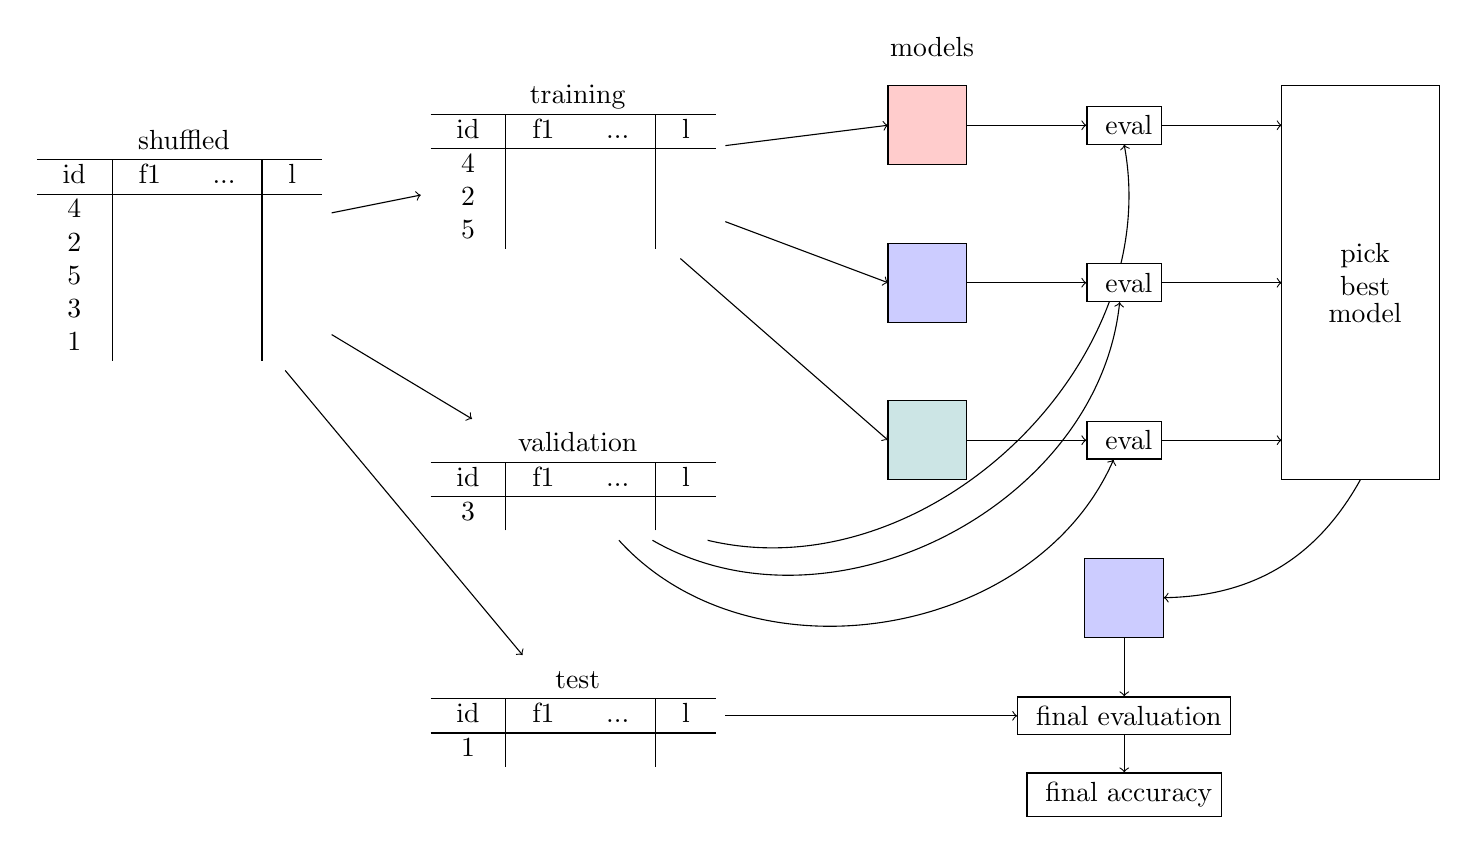
\begin{tikzpicture}
                        \node (shuffled) at (0, 0) {
                            \begin{tabular}{c|cc|c}
                                \multicolumn{4}{c}{~shuffled~} \\
                                \hline
                                ~id~ & ~f1~ & ~...~ & ~l~ \\
                                \hline
                                4 & & & \\
                                2 & & & \\
                                5 & & & \\
                                3 & & & \\
                                1 & & & \\
                            \end{tabular}
                        };
                        \node (training) at (5, 1) {
                            \begin{tabular}{c|cc|c}
                                \multicolumn{4}{c}{~training~} \\
                                \hline
                                ~id~ & ~f1~ & ~...~ & ~l~ \\
                                \hline
                                4 & & & \\
                                2 & & & \\
                                5 & & &
                            \end{tabular}
                        };
                        \node (validation) at (5, -3) {
                            \begin{tabular}{c|cc|c}
                                \multicolumn{4}{c}{~validation~} \\
                                \hline
                                ~id~ & ~f1~ & ~...~ & ~l~ \\
                                \hline
                                3 & & &
                            \end{tabular}
                        };
                        \node (test) at (5, -6) {
                            \begin{tabular}{c|cc|c}
                                \multicolumn{4}{c}{~test~} \\
                                \hline
                                ~id~ & ~f1~ & ~...~ & ~l~ \\
                                \hline
                                1 & & &
                            \end{tabular}
                        };

                        \node (eval0) at (12, 1.5) {~eval~};
                        \node (eval1) at (12, -0.5) {~eval~};
                        \node (eval2) at (12, -2.5) {~eval~};
                        \node[draw] (fe) at (12, -6) {~final evaluation~};
                        \node[draw] (fa) at (12, -7) {~final accuracy~};

                        \draw
                        (shuffled) edge[->] (training)
                        (shuffled) edge[->] (validation)
                        (shuffled) edge[->] (test)
                        (training) edge[->] (9, 1.5)
                        (training) edge[->] (9, -0.5)
                        (training) edge[->] (9, -2.5)
                        (validation) edge[bend right=57, ->] (eval0)
                        (validation) edge[bend right=57, ->] (eval1)
                        (validation) edge[bend right=57, ->] (eval2)
                        (9, 1.5) edge[->] (eval0)
                        (9, -0.5) edge[->] (eval1)
                        (9, -2.5) edge[->] (eval2)
                        (eval0) edge[->] (14, 1.5)
                        (eval1) edge[->] (14, -0.5)
                        (eval2) edge[->] (14, -2.5)
                        (15, -3) edge[bend left=30, ->] (12.5, -4.5)
                        (12, -5) edge[->] (fe)
                        (test) edge[->] (fe)
                        (fe) edge[->] (fa);

                        \node[draw, fill=white] (eval0) at (12, 1.5) {~eval~};
                        \node[draw, fill=white] (eval1) at (12, -0.5) {~eval~};
                        \node[draw, fill=white] (eval2) at (12, -2.5) {~eval~};

                        \node at (9.5, 2.5) {~models~};
                        \node at (15, -0.5) {\shortstack{~pick~\\~best~\\~model~}};

                        \draw (14, 2) -- (16, 2) -- (16, -3) -- (14, -3) -- cycle;

                        \draw[fill=red!20] (9, 2) -- (10, 2) -- (10, 1) -- (9, 1) -- cycle;
                        \draw[fill=blue!20] (9, 0) -- (10, 0) -- (10, -1) -- (9, -1) -- cycle;
                        \draw[fill=teal!20] (9, -2) -- (10, -2) -- (10, -3) -- (9, -3) -- cycle;
                        \draw[fill=blue!20] (11.5, -4) -- (12.5, -4) -- (12.5, -5) -- (11.5, -5) -- cycle;
                    \end{tikzpicture}
                \end{center}
            \subsubsection*{Cross-validation}
                The idea of cross-validation is that the dataset can be divided into $k$ (usually 10) equal splits.
                $k - 1$ of these folds can be used for training and validation, and the remaining split can be used for testing.
                This is done $k$ times, each time testing on a different portion of the data, in which we test on all of the data (but notice we never train and test on the same data at the same time).
                The performance on all $k$ held-out test sets can be averaged;
                $$\text{global error estimate } = \frac{1}{N}\summation{i=1}{N} e_i$$
                Note that this is used to evaluate an algorithm, not a particular model.
                \medskip

                This method needs to be slightly modified when doing parameter tuning, in which we have the following options;
                \begin{enumerate}[{option} 1:]
                    \itemsep0em
                    \item
                        At each iteration, we use 1 fold for testing, 1 for validation, and the remaining $k - 2$ folds for training.
                        However, this will give us a different set of optimal parameters in each fold.
                    \item
                        Another approach is to do cross-validation within cross-validation.
                        As before, we still separate 1 fold for testing, however we run another internal cross-validation over the remaining $k - 1$ folds to obtain the optimal hyperparameters.
                        Once we obtain the best hyperparameters, we can then test it against the fold reserved for testing to obtain the final evaluation.
                        This isn't always practical, as it requires a lot of computation for complex models.
                \end{enumerate}
                When we go into production (not as common in academia), we may use all the remaining reserved test data for training as well (once we have the optimal parameters).
                However, this comes with the downside that we are no longer able to estimate the performance of the final trained model.
            \subsubsection*{Performance Metrics}
                Once we have a model, we want to have a quantifiable way to judge the quality of a model against another.
                Consider the following results from the test dataset;
                \begin{center}
                    \hfill
                    \begin{tabular}{c|cc}
                        id & label & prediction \\
                        \hline
                        ~1~ & ~+~ & ~+~ \\
                        ~2~ & ~+~ & ~+~ \\
                        ~3~ & ~+~ & ~-~ \\
                        ~4~ & ~+~ & ~+~ \\
                        ~5~ & ~-~ & ~-~ \\
                        ~6~ & ~-~ & ~+~ \\
                        ~7~ & ~-~ & ~-~ \\
                        ~8~ & ~-~ & ~+~
                    \end{tabular}
                    \hfill
                    \begin{tabular}{c|cc}
                        & class 1 (predicted) & class 2 (predicted) \\
                        \hline
                        class 1 (actual) & true positive (3) & false negative (1) \\
                        class 2 (actual) & false positive (2) & true negative (2)
                    \end{tabular}
                    \hfill \phantom{}
                \end{center}
                This confusion matrix highlights the risk of each prediction - sometimes it can be more important to have fewer false negatives than fewer false positives (such as diagnosing a disease)
                It also allows for easy identification of confusion between classes (when one class is commonly mislabelled as another).
                Many other measures can be computed from the confusion matrix.
                In our example, we have two classes (positive and negative).
                The common measures are as follows;
                \begin{itemize}
                    \itemsep0em
                    \item \textbf{accuracy} \hfill $\frac{TP + TN}{TP + TN + FP + FN}$
                        \subitem
                            This is simply the number of correctly classified examples divided by the total number of examples.
                            The classification error is $1 - \text{accuracy}$.
                    \item \textbf{precision} \hfill $\frac{TP}{TP + FP}$
                        \subitem
                            This is the number of correctly classified positive examples divided by the total number of predicted positive examples.
                            We can also think about it as;
                            $$P(~positive~\ \vline\ ~example classified as positive~)$$
                            A high precision implies that an example labelled as positive is actually positive (few false positives).
                    \item \textbf{recall} \hfill $\frac{TP}{TP + FN}$
                        \subitem
                            This can be considered as the inverse of precision.
                            It is the number of correctly classified positive examples divided by the number of actual positive examples.
                            It can be thought of as
                            $$P(~correctly classified as positive~\ \vline\ ~actually positive~)$$
                            A high recall implies that the class is correctly recognised (therefore a small number of false negatives).
                    \item \textbf{F-measure / F-score} \hfill $F_1 = \frac{2 \cdot ~precision~ \cdot ~recall~}{~precision~ + ~recall~}$
                        \subitem
                            Sometimes it is useful to measure the performance of the classifier with a single number.
                            More generally it can be written as (with more emphasis on precision for higher $\beta$);
                            $$F_\beta = (1 + \beta^2) \cdot \frac{~precision~ \cdot ~recall~}{(\beta^2 \cdot ~precision~) + ~recall~}$$
                \end{itemize}
                For something to be high recall and low precision, most of the positive examples are correctly recognised, but with many false positives.
                On the other hand if something has low recall and high precision, we miss a lot of positive examples, but the ones that we predict as positive are more likely to be actually positive.
                \medskip

                The macro-averaged recall is the mean of the recalls for all the classes.
                The same can be done for precision and F-measure.
                In the multi-class case, precision, recall, and F-measure are computed for each class separately (we define one class each time as being the positive class).
                Note that macro-averaging is done on the class level, and is the average of the metrics for each class.
                On the other hand, micro-averaging does it on the item level (adding the TP, FP, TN, FN values for each class before calculating the metrics).
                Note that micro-averaged P, R and F1 will be equal to accuracy.
                \medskip

                Another measure is regression tasks, where a lower mean squared error (MSE) is better (where $Y_i$ is a sample from the dataset and $\hat{Y}_i$ is the prediction from the model);
                $$\frac{1}{N} \summation{i = 1}{N} (Y_i - \hat{Y}_i)^2$$
                However, we don't only care about accuracy, our models should be;
                \begin{itemize}
                    \itemsep0em
                    \item \textbf{accurate} \hfill makes correct predictions
                    \item \textbf{fast} \hfill fast to train and query
                    \item \textbf{scalable} \hfill works with large datasets
                    \item \textbf{simple} \hfill understandable and robust
                    \item \textbf{interpretable} \hfill can explain predictions
                \end{itemize}
            \subsubsection*{Imbalanced Datasets}
                In a balanced dataset, we have an equal number of positive and negative data points.
                However, this will not always be the case, and we may have an unbalanced dataset where classes are not equally represented.
                The accuracy goes down, as it tends to follow the majority class.
                Additionally, the precision may also go down for the minority class.
                Consider the following case;
                \begin{center}
                    \begin{tabular}{c|cc}
                        & class 1 (predicted) & class 2 (predicted) \\
                        \hline
                        class 1 (actual) & 700 & 300 \\
                        class 2 (actual) & 100 & 0
                    \end{tabular}
                \end{center}
                From this, we obtain the following metrics where the accuracy may be high, but class 2 is completely misclassified;
                \begin{align*}
                    R(c1) & = 0.7 \\
                    P(c1) & = 0.875 \\
                    F_1(c1) & \approx 0.778 \\
                    R(c2) & = 0 \\
                    P(c2) & = 0 \\
                    F_1(c2) & = ~N/A~ \\
                    A & \approx 0.636
                \end{align*}
                In conclusion, we need to look at different metrics, as well as the confusion matrix as a single metric may be misleading by itself.
                \medskip

                We can normalise the confusion matrix by dividing each member of a row by the sum of that row (such that each row adds to one).
                We can also downsample the majority class, by picking less examples to get the two classes equal, or upsample the minority class by duplicating data.
                Neither will reflect how the model will generalise.
            \subsubsection*{Overfitting}
                An overfitted model has good performance on training data, but poor generalisation to other data.
                On the other hand, underfitting has poor performance on the training data, as well as poor generalisation.
                \begin{center}
                    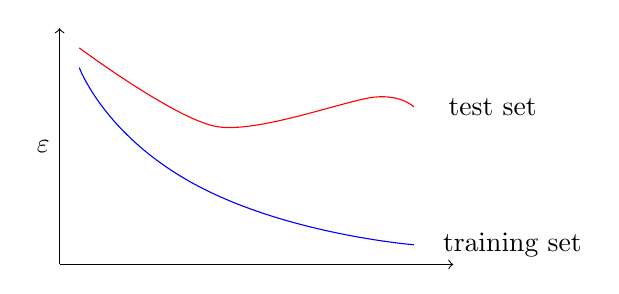
\begin{tikzpicture}
                        \draw
                        (0, 0) edge[->, left] node{$\varepsilon$} (0, 3)
                        (0, 0) edge[->] (5, 0);

                        \draw [red] plot [smooth] coordinates { (0.25, 2.75) (2, 1.75) (4, 2.125) (4.5, 2) };
                        \draw [blue] plot [smooth, tension=1] coordinates { (0.25, 2.5) (1.75, 1) (4.5, 0.25) };

                        \node at (5.5, 2) {test set};
                        \node at (5.75, 0.25) {training set};
                    \end{tikzpicture}
                \end{center}
                In the example above, it starts off with an underfitted model, and then ends up overfitted.
                The point where it's correct is just as the error of the test set begins to increase again.
                \medskip

                Overfitting can occur under these scenarios (and how we could avoid it);
                \begin{itemize}
                    \itemsep0em
                    \item model used is too complex (learns too many fine details)
                        \subitem use the validation set to decide the complexity
                    \item examples in the training set are not representative of all possible situations
                        \subitem obtain more data
                    \item learning is performed for too long (such as neural networks)
                        \subitem stopping the training earlier (using the validation set to decide when)
                \end{itemize}
            \subsubsection*{Confidence Intervals}
                The amount of data used in our test set also affects our confidence of the performance evaluation.
                A 90\% accuracy score on a test set with 10 samples is still less trustworthy than an 84\% accuracy score on a test set with 10,000 samples.
                \medskip

                We define the true error of the model $h$ as the probability that it will misclassify a randomly drawn example $x$ from distribution $D$;
                $$error_D(h) \equiv P[f(x) \neq h(x)]$$
                The \textbf{sample error} of the model $h$ based on a data sample $S$ is as follows;
                \begin{align*}
                    n & = \text{number of samples} \\
                    \delta(f(x), h(x)) & = \begin{cases}
                        1 & f(x) \neq h(x) \\
                        0 & f(x) = h(x)
                    \end{cases} \\
                    error_S(h) & \equiv \frac{1}{n} \summation{x \in S}{} \delta(f(x), h(x))
                \end{align*}
                We can say an $N\%$ confidence interval for some parameter $q$ is an interval with probability $N$ to contain the true value of $q$.
                Given a sample $S$, with more than 30 examples;
                $$error_S(h) \pm Z_N \underbrace{\sqrt{\frac{error_S(h) \cdot (1 - error_S(h))}{n}}}_\text{est. standard deviation of sample error}$$
                Due to the $n$ in the estimation of the standard deviation, if we have a very large $n$, we can obtain a very tight confidence interval.
                An example of this applied is as follows;
                \medskip

                Emotion recognition results for 3 samples, using 156 training and 50 testing samples.
                \begin{center}
                    \begin{tabular}{lllll}
                        & attributes & number of classes & classifier & correctly classified \\
                        \hline
                        face & 67 * 8 & C4.5 & 78\% \\
                        body & 140 & 6 & BayesNet & 90\%
                    \end{tabular}
                \end{center}
                We want to classify the 95\% confidence interval for this error ($Z_N = 1.96$)
                \begin{align*}
                    error_S(h) & = 0.22 \\
                    n & = 50 \\
                    Z_N & = 1.96 \\
                    \text{interval} & = \left[0.22 - 1.96\sqrt{\frac{0.22 \cdot (1 - 0.22)}{50}}, 0.22 + 1.96\sqrt{\frac{0.22 \cdot (1 - 0.22)}{50}}\right] \\
                    & = [0.11, 0.33]
                \end{align*}
            \subsubsection*{Significance Testing}
                Statistical tests can tell us if the means of two sets are significantly different;
                \begin{itemize}
                    \itemsep0em
                    \item \textbf{randomisation test}
                        \subitem
                            Randomly switch some predictions between two models and measure if the performance difference that we get is greater than or equal to the original difference.
                    \item \textbf{two-sample T-test}
                        \subitem
                            This is used to estimate if two metrics from different populations are actually different.
                            This has lower computational requirements and is easier to calculate.
                    \item \textbf{paired T-test}
                        \subitem
                            Examining significance over multiple matched results, such as classification error over the same folds in cross-validation.
                \end{itemize}
                The \textbf{null hypothesis} (see \textbf{CO245}) is the hypothesis that the two algorithms / models perform the same and the differences are only due to sampling error.
                These tests return a \textbf{p-value}, which is the probability of obtaining the differences we see, assuming the null hypothesis is correct.
                A small p-value implies that we can be more confident that one system is actually different.
                \medskip

                We consider a performance difference to be \textbf{statistically significant} of $p < 0.05$.
                However, $p > 0.05$ does not mean the algorithms are similar, just that we cannot observe a statistical difference.
                \medskip

                There's a fairly long bit on \textbf{P-hacking}, but not sure why.
                A way to protect against P-hacking is to use an adaptive p-value;
                \begin{enumerate}[1.]
                    \itemsep0em
                    \item rank p-values from $M$ experiments;
                        $$p_1 \leq p_2 \leq p_3 \leq \dots \leq p_M$$
                    \item calculate the \textbf{Benjamini-Hochberg} critical value for each experiment;
                        $$z_i = 0.05 \frac{i}{M}$$
                    \item significant results are the ones where the p-value is smaller than the critical value
                \end{enumerate}
        \subsection*{Week 5 (Artificial Neural Networks I)}
        \subsection*{Week 6 (Artificial Neural Networks II)}
        \subsection*{Week 7 (Unsupervised Learning)}
        \subsection*{Week 8 (Genetic Algorithms)}
\end{document}